\section{Software Deployment Strategy}\label{sect:deploy}
The LSST software deployment strategy follows a continuous integration (CI) process to support development all the way to 
deployment, employing industry standard tools. Figure~\ref{fig:deploy} shows a diagram with the process. This process 
applies to all software component of the system infrastructure, from SAL and CSCs (regardless of the 
programing language they are written in) to SAL Scripts and all the other libraries. 

\begin{figure}
\begin{center}
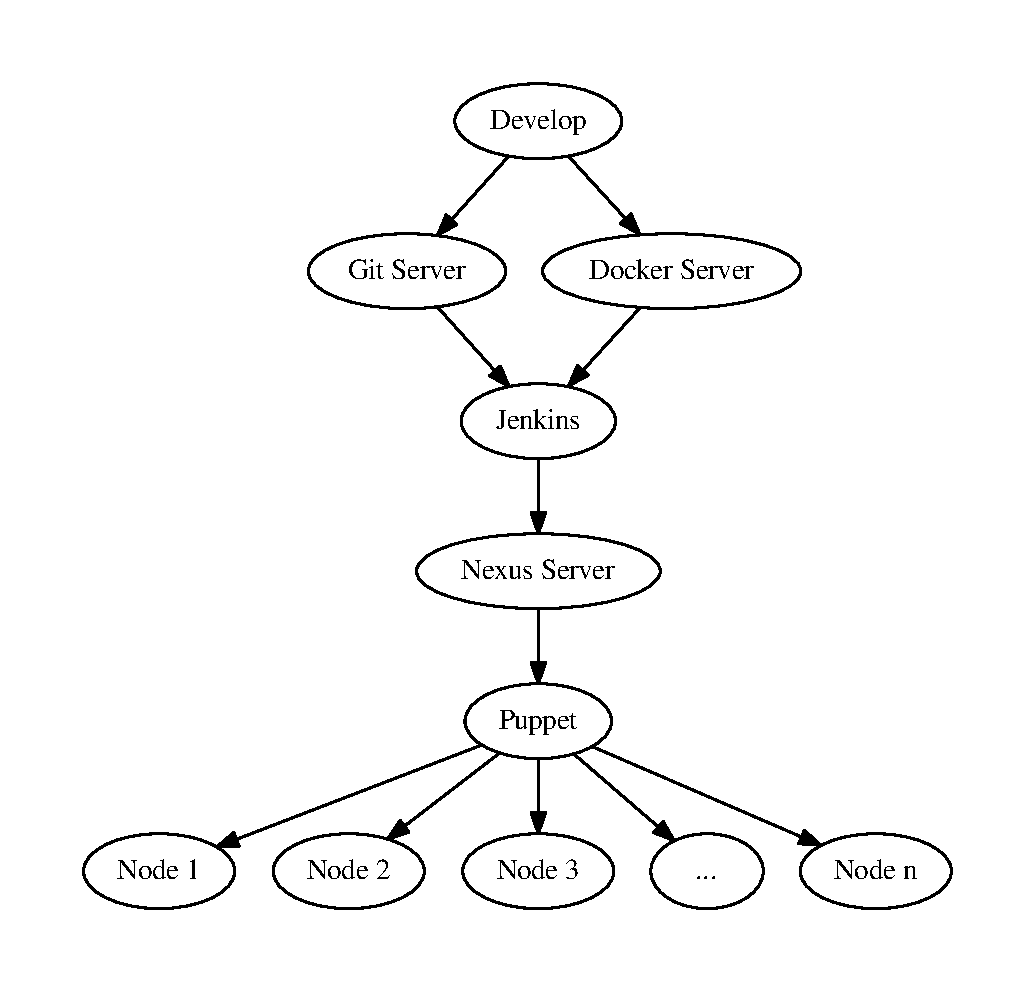
\includegraphics[width=0.55\textwidth]{deploy}
\caption{Diagram outlining the software deployment strategy.\label{fig:deploy}}
\end{center}
\end{figure}

As one can see from Fig.~\ref{fig:deploy}, the main end solution to the deployment strategy is the use of Puppet. Puppet is 
an open source systems management tool for centralized and automated configuration management. The main idea behind 
this service is that it is possible to describe the system architecture (e.g. how the "system should be") in a configuration
file. Then the server is capable of configuring each node with the appropriate software. 

The choice of a "configuration management" or "deployment system" (e.g. Puppet) still leaves open the question of how the 
software is packaged. One of the largest growing and broadly used industry-standard solutions in use for distributed systems 
like the LSST, is Docker. Docker is a container solution for software deployment, which packs code and all its 
dependencies into a lightweight virtual machine-like environment. It also runs quickly and reliably from one computing 
environment to another. 

Development is the first stage of the process and is where code is either created (e.g. new CSCs, new scripts being 
developed, etc) or modified (e.g. bug fixes, improvements, etc). Once development is completed and the software is tested 
and validated it goes to the Git Server. At this stage, a Docker image may also be created and stored in the Docker Server. 
Once this is completed a Jenkins build is triggered. For the build, Jenkins will pull the software, along with all its 
dependencies, build and run unit and integration tests. If all tests passes, the software is then packed by Jenkins; 
which may be a new Docker image with the new version of the code, an RPM package or some other package 
method that can be used by Puppet. The software package is then sent to the Nexus Server. 

In some cases, the resulting Docker image to contain the software may exceed Jenkins build size limit, and it is not 
capable of creating images for testing and deployment to the Nexus Server. In these cases, the developer creates the 
Docker image and place it in the Docker Server. Jenkins will pull the Docker image, start it locally and run the unit and 
integrations tests. If the test passes, Jenkins pushes the image to the Nexus Server.

Once the final version of the software is packed and stored in the Nexus Server, Puppet can be instructed to update the 
software on a specific node (or nodes). 

